%!TEX root = ../Thesis.tex
%\chapter{Long chapter title with $\pi$ $π$ or π}
%\chapter{Long chapter title with \texorpdfstring{$\pi$ $π$ or π}{π π or π}}
\section{Including Physics in Deep Learning – An Example from 4D Seismic Pressure Saturation Inversion}

\paragraph{Abstract:} Geoscience data often have to rely on strong priors in the face of uncertainty. Additionally, we often try to detect or model anomalous sparse data that can appear as an outlier in machine learning models. These are classic examples of imbalanced learning. Approaching these problems can benefit from including prior information from physics models or transforming data to a beneficial domain. We show an example of including physical information in the architecture of a neural network as prior information. We go on to present noise injection at training time to successfully transfer the network from synthetic data to field data.
\vfill
\subsection*{Key points:}
\begin{itemize}
    \item \acl{dnn} to invert seismic for pressure-saturation data
    \item Compared to Bayesian inversion
    \item Indicators for good performance:
    \subitem Context-unaware network results have spatial consistency
    \subitem Values unconstrained but predict correct range
    \subitem Areas of effect match prediction
    \item Training on simulation data transfers to field data
\end{itemize}
\vfill
{\vfill\hfill\newline\fbox{\parbox{.97\textwidth}{\fullcite{dramsch2019including}}}}

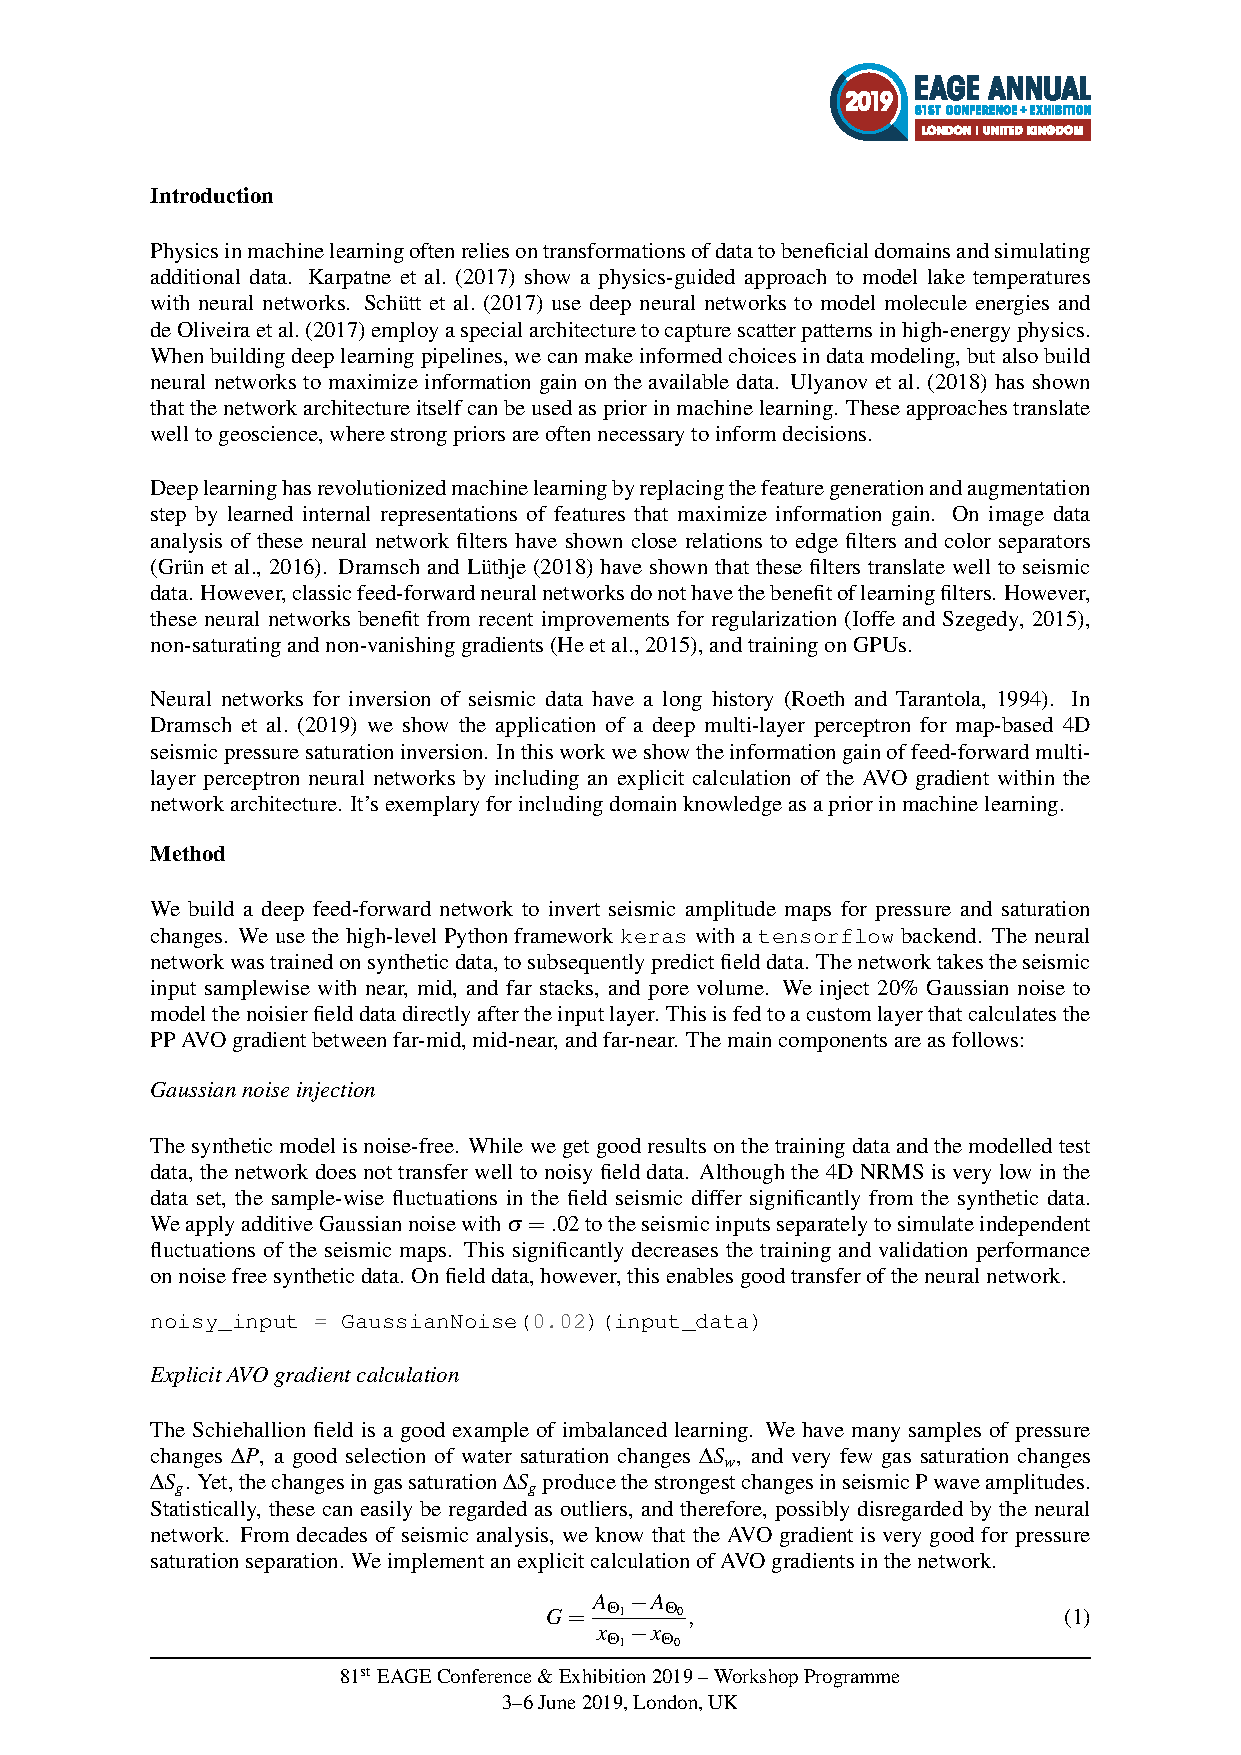
\includepdf[pages={1-4},pagecommand={},width=1.2\textwidth,offset=0.7cm -1.5cm]{papers/2019.3}